\section[ML overview]{Machine learning overview}

\subsection{}

\begin{frame}
    \frametitle{What is machine learning?}

    \begin{block}{My definition}
        The study of computational algorithms
        \begin{itemize}
            \item that \alert{predict} outputs from inputs;
            \item whose behavior is determined by \alert{model parameters};
            \item that \alert{learn} how to make predictions by fitting (``training'') the model parameters to data;
            \item that \alert{iteratively} improve their model parameters via continual training.
        \end{itemize}
    \end{block}

    \begin{columns}
        \begin{column}{2.5in}
            Simplest example: linear regression
            \begin{itemize}
                \item Sort of: not iterative
                \item Predicts $y$ from $x$ via $y = ax + b$
                \item Two parameters: $a$, $b$
                \item Fitted to data
            \end{itemize}
        \end{column}
        \begin{column}{1.75in}
            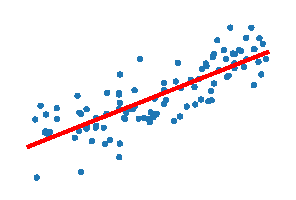
\includegraphics{linear_regression}
        \end{column}
    \end{columns}
\end{frame}

\begin{frame}
    \frametitle{A (much) more complicated example}
    \begin{columns}
        \begin{column}{0.37\textwidth}
            \begin{block}{Image classification}
                A canonical problem: given an image, predict the correct label
            \end{block}
        \end{column}
        \begin{column}{0.63\textwidth}
            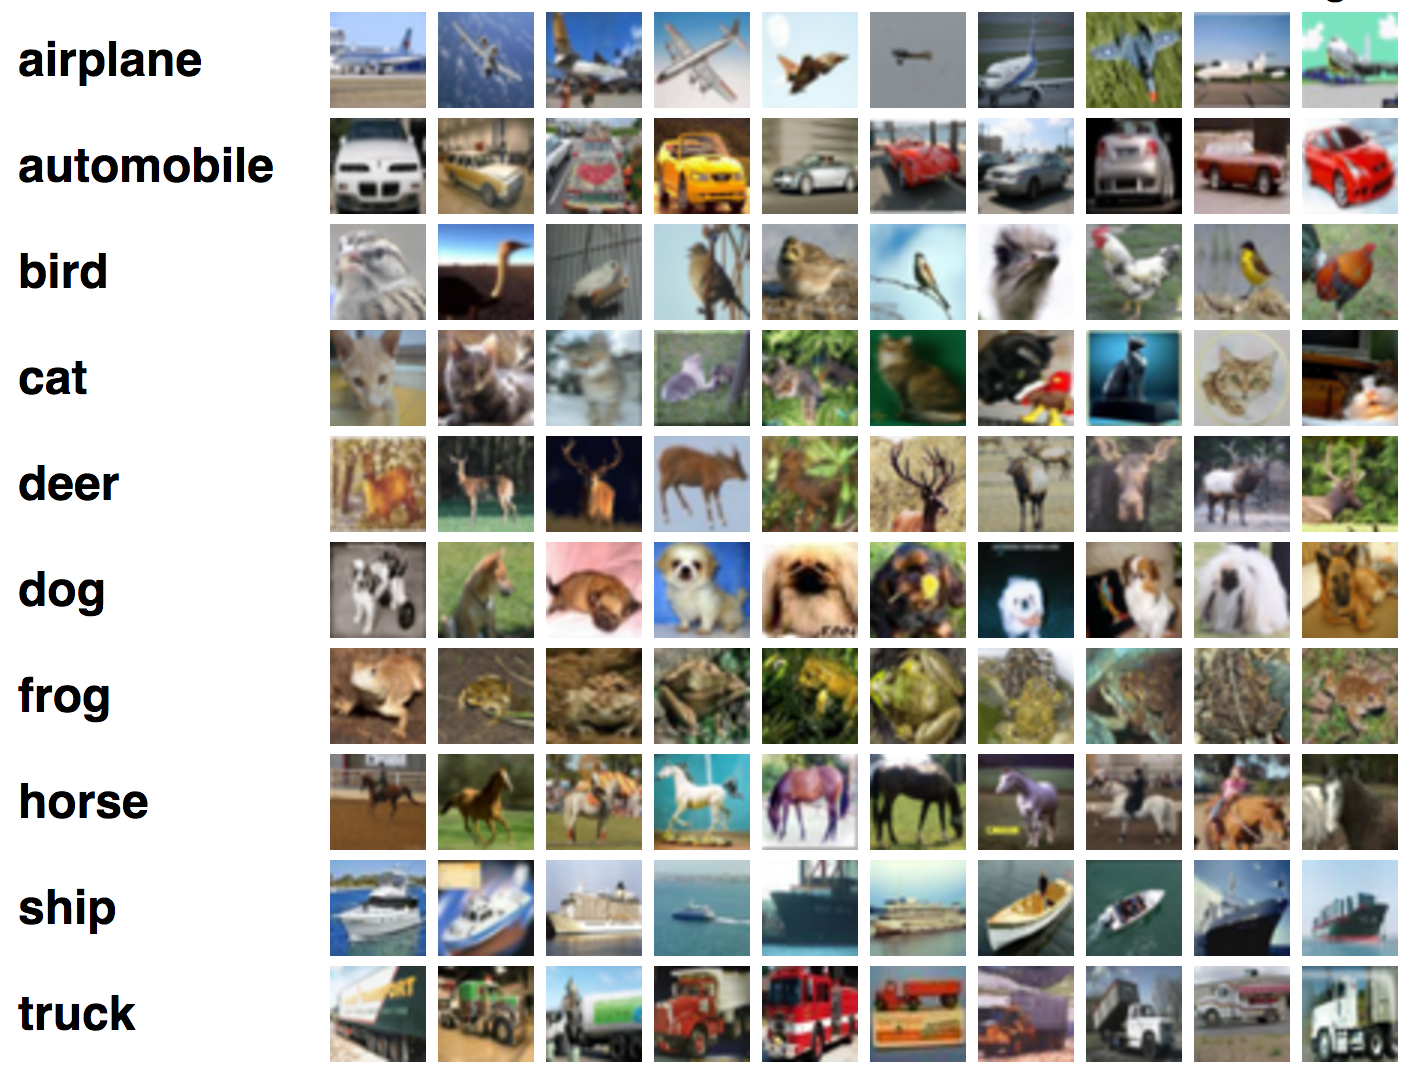
\includegraphics[width=\textwidth]{cifar10}
        \end{column}
    \end{columns}

    \begin{itemize}
        \item Roughly: if a human can do it, a computer should be able to too
        \item More rigorously: $\exists$ a mapping from image pixels to labels
        \begin{itemize}
            \item Mapping too difficult for humans to understand
            \item Let an algorithm model it
        \end{itemize}
    \end{itemize}
\end{frame}

\begin{frame}
    \frametitle{An image classification solution}

    \begin{columns}
        \begin{column}{0.7\textwidth}
            ResNet-152: a 152-layer convolutional neural network with 11.3 billion multiply/adds! \citep{He15}
            \begin{itemize}
                \item Trained on ImageNet data: 14,197,122 images
                \item Iterative training
                \begin{itemize}
                    \item 600,000 training iterations
                    \item At each iteration, model parameters updated based on \emph{mini-batch} of 256 images
                \end{itemize}
                \item Won multiple image classification competitions
            \end{itemize}
        \end{column}
        \begin{column}{0.3\textwidth}
            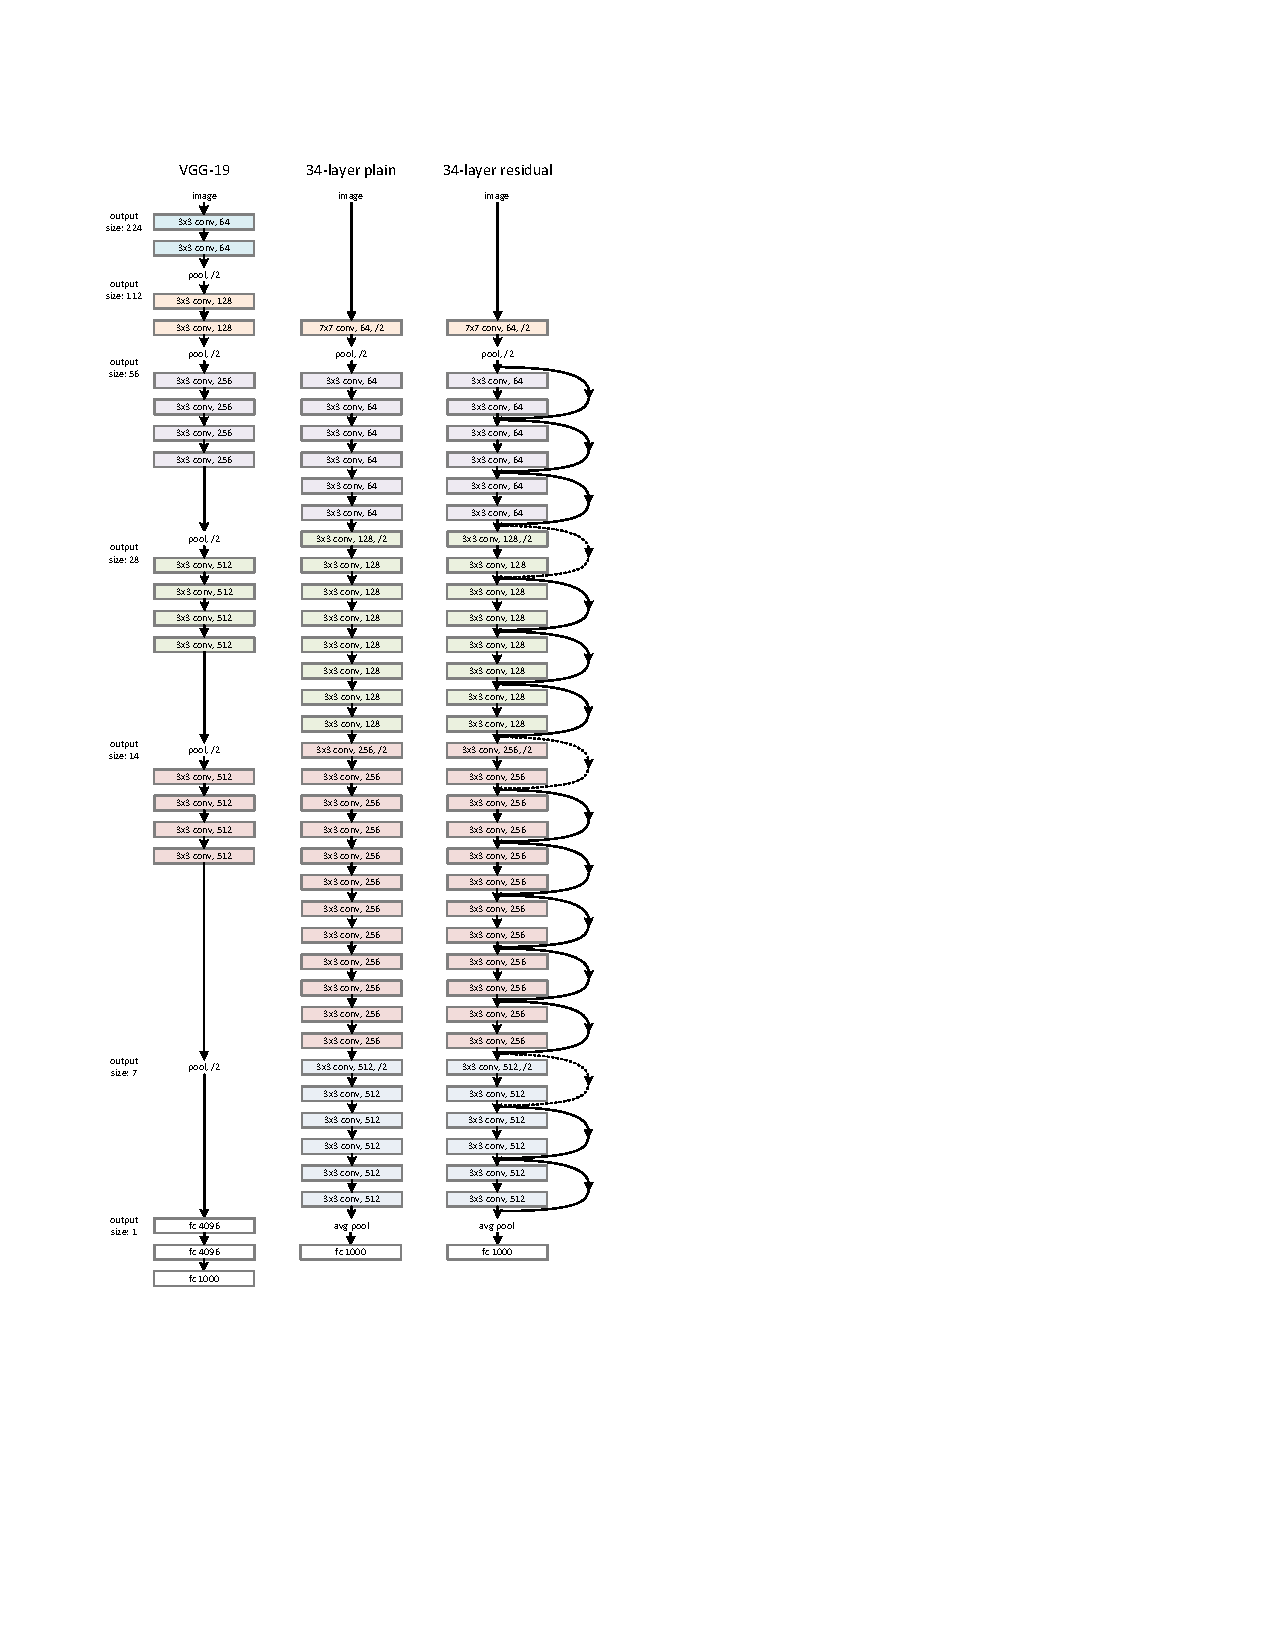
\includegraphics[width=\textwidth]{resnet}
        \end{column}
    \end{columns}
\end{frame}

\begin{frame}
    \frametitle{Converting classification to regression: one-hot}

    Classification problems almost always converted to regression via easy trick

    \begin{block}{One-hot encoding}
        For labels $1, \dots, n$, represent each label as the unit vector $\e_i$, $i = 1, \dots, n$ \\[1ex]
        One-hot vectors loosely interpreted as
        \begin{equation*}
            \begin{bmatrix}
                \P(\text{label} = 1) & \cdots & \P(\text{label} = n)
            \end{bmatrix}
        \end{equation*}
    \end{block}

    E.g. image classification: \\[0.5ex]

    \centering
    \begin{tabular}{c|cc}
        label & index & one-hot vector \\
        \hline
        bird & 1 & $\begin{bmatrix} 1 & 0 & 0 & 0 & \cdots & 0 \end{bmatrix}$ \\
        cat & 2 & $\begin{bmatrix} 0 & 1 & 0 & 0 & \cdots & 0 \end{bmatrix}$ \\
        dog & 3 & $\begin{bmatrix} 0 & 0 & 1 & 0 & \cdots & 0 \end{bmatrix}$ \\
    \end{tabular}
\end{frame}

\begin{frame}
    \frametitle{Converting classification to regression: softmax}
    One-hot works for labeling data.
    What about model outputs?

    \begin{block}{Softmax activation}
        Converts arbitrary real vector (called \textcolor{blue}{logits}) to \textcolor{Green4}{vector of probabilities that sums to 1}
        \vspace{-1pt}
        \begin{align*}
            \softmax &: \textcolor{blue}{\Reals^n} \to
            \textcolor{Green4}{(0, 1)^n \text{ with } L^1 \text{ norm} = 1} \\
            &\hspace{1.25ex} \textcolor{blue}{%
                \left(\begin{bmatrix} y_1 & \cdots & y_n \end{bmatrix}\right)%
            } \mapsto
            \textcolor{Green4}{%
                \frac{1}{\sum_{i=1}^n e^{y_i}}
                \begin{bmatrix}
                    e^{y_1} & \cdots & e^{y_n}
                \end{bmatrix}%
            }
        \end{align*}
        \vspace{-1pt}
        Like one-hot, output loosely interpreted as
        \vspace{-1pt}
        \begin{equation*}
            \textcolor{Green4}{%
                \begin{bmatrix}
                    \P(\text{label} = 1) & \cdots & \P(\text{label} = n)
                \end{bmatrix}%
            }
        \end{equation*}
    \end{block}

    \begin{itemize}
        \item E.g.: model outputs \textcolor{blue}{%
            logits
            $\y = \begin{bmatrix} -3.33 & 9.62 & 9.18 & \cdots \end{bmatrix}$
        }
        \item \textcolor{Green4}{%
            $\softmax(\y) = \begin{bmatrix} 1.40\E{-6} & 0.593 & 0.381 & \cdots \end{bmatrix}$
        }
        \item Model is 59.3\% confident in ``cat,'' 38.1\% confident in ``dog''
    \end{itemize}
\end{frame}

%%% Local Variables:
%%% mode: latex
%%% TeX-master: "../nn"
%%% End:
